\documentclass[a0]{sciposter}

% ******************************************************************************
% ****************************** Custom Margin *********************************

% Add `custommargin' in the document class options to use this section
% Set {innerside margin / outerside margin / topmargin / bottom margin}  and
% other page dimensions
\ifsetCustomMargin
  \RequirePackage[left=37mm,right=30mm,top=35mm,bottom=30mm]{geometry}
  \setFancyHdr % To apply fancy header after geometry package is loaded
\fi

% *****************************************************************************
% ******************* Fonts (like different typewriter fonts etc.)*************

% Add `customfont' in the document class option to use this section

\ifsetCustomFont
  % Set your custom font here and use `customfont' in options. Leave empty to
  % load computer modern font (default LaTeX font).
  % \RequirePackage{helvet}
  \usepackage{helvet}
  \renewcommand{\familydefault}{\sfdefault}
\fi

% *****************************************************************************
% **************************** Custom Packages ********************************

% ************************* Algorithms and Pseudocode **************************

%\usepackage{algpseudocode}


% ********************Captions and Hyperreferencing / URL **********************

% Captions: This makes captions of figures use a boldfaced small font.
%\RequirePackage[small,bf]{caption}

\RequirePackage[labelsep=space,tableposition=top]{caption}
\renewcommand{\figurename}{Fig.} %to support older versions of captions.sty


% *************************** Graphics and figures *****************************

%\usepackage{rotating}
%\usepackage{wrapfig}

% Uncomment the following two lines to force Latex to place the figure.
% Use [H] when including graphics. Note 'H' instead of 'h'
%\usepackage{float}
%\restylefloat{figure}

% Subcaption package is also available in the sty folder you can use that by
% uncommenting the following line
% This is for people stuck with older versions of texlive
%\usepackage{sty/caption/subcaption}
\usepackage{subcaption}

% ********************************** Tables ************************************
\usepackage{booktabs} % For professional looking tables
\usepackage{multirow}

%\usepackage{multicol}
%\usepackage{longtable}
%\usepackage{tabularx}


% ***************************** Math and SI Units ******************************

\usepackage{amsfonts}
\usepackage{amsmath}
\usepackage{amssymb}
\usepackage{siunitx} % use this package module for SI units


% ******************************* Line Spacing *********************************

% Choose linespacing as appropriate. Default is one-half line spacing as per the
% University guidelines

% \doublespacing
% \onehalfspacing
% \singlespacing


% ************************ Formatting / Footnote *******************************

% Don't break enumeration (etc.) across pages in an ugly manner (default 10000)
%\clubpenalty=500
%\widowpenalty=500

%\usepackage[perpage]{footmisc} %Range of footnote options


% *****************************************************************************
% *************************** Bibliography  and References ********************

%\usepackage{cleveref} %Referencing without need to explicitly state fig /table

% Add `custombib' in the document class option to use this section
\ifuseCustomBib
   \RequirePackage[square, sort, numbers, authoryear]{natbib} % CustomBib

% If you would like to use biblatex for your reference management, as opposed to the default `natbibpackage` pass the option `custombib` in the document class. Comment out the previous line to make sure you don't load the natbib package. Uncomment the following lines and specify the location of references.bib file

%\RequirePackage[backend=biber, style=numeric-comp, citestyle=numeric, sorting=nty, natbib=true]{biblatex}
%\bibliography{References/references} %Location of references.bib only for biblatex

\fi

% changes the default name `Bibliography` -> `References'
\renewcommand{\bibname}{References}


% *****************************************************************************
% *************** Changing the Visual Style of Chapter Headings ***************
% This section on visual style is from https://github.com/cambridge/thesis

% Uncomment the section below. Requires titlesec package.

%\RequirePackage{titlesec}
%\newcommand{\PreContentTitleFormat}{\titleformat{\chapter}[display]{\scshape\Large}
%{\Large\filleft{\chaptertitlename} \Huge\thechapter}
%{1ex}{}
%[\vspace{1ex}\titlerule]}
%\newcommand{\ContentTitleFormat}{\titleformat{\chapter}[display]{\scshape\huge}
%{\Large\filleft{\chaptertitlename} \Huge\thechapter}{1ex}
%{\titlerule\vspace{1ex}\filright}
%[\vspace{1ex}\titlerule]}
%\newcommand{\PostContentTitleFormat}{\PreContentTitleFormat}
%\PreContentTitleFormat


% ******************************************************************************
% ************************* User Defined Commands ******************************
% ******************************************************************************

% *********** To change the name of Table of Contents / LOF and LOT ************

%\renewcommand{\contentsname}{My Table of Contents}
%\renewcommand{\listfigurename}{My List of Figures}
%\renewcommand{\listtablename}{My List of Tables}


% ********************** TOC depth and numbering depth *************************

\setcounter{secnumdepth}{2}
\setcounter{tocdepth}{2}


% ******************************* Nomenclature *********************************

% To change the name of the Nomenclature section, uncomment the following line

%\renewcommand{\nomname}{Symbols}


% ********************************* Appendix ***********************************

% The default value of both \appendixtocname and \appendixpagename is `Appendices'. These names can all be changed via:

%\renewcommand{\appendixtocname}{List of appendices}
%\renewcommand{\appendixname}{Appndx}

% ******************************** Draft Mode **********************************

% Uncomment to disable figures in `draftmode'
%\setkeys{Gin}{draft=true}  % set draft to false to enable figures in `draft'

% These options are active only during the draft mode
% Default text is "Draft"
%\SetDraftText{DRAFT}

% Default Watermark location is top. Location (top/bottom)
%\SetDraftWMPosition{bottom}

% Draft Version - default is v1.0
%\SetDraftVersion{v1.1}

% Draft Text grayscale value (should be between 0-black and 1-white)
% Default value is 0.75
%\SetDraftGrayScale{0.8}


%% Todo notes functionality
%% Uncomment the following lines to have todonotes.

%\ifsetDraft
%   \usepackage[colorinlistoftodos]{todonotes}
%   \newcommand{\mynote}[1]{\todo[author=kks32,size=\small,inline,color=green!40]{#1}}
%\else
%   \newcommand{\mynote}[1]{}
%   \newcommand{\listoftodos}{}
%\fi

% Example todo: \mynote{Hey! I have a note}


\begin{document}
    \begin{center}
    
\includegraphics[width=0.15\textwidth]{Unibersidad_ng_Pilipinas}
    \par\Large\MakeUppercase{\textbf{Crime Modeling and Prediction using Recurrent Neural Networks with Long Short-term Memory Architecure}}
    \par Jay Arnel D. Bilocura, Kurt Junshean P. Espinosa
    \par Machine Learning Group, Department of Computer Science
    \par University of the Philippines Cebu
    \par \{jdbilocura, kpespinosa\}@up.edu.ph
    \end{center}
    \begin{multicols}{2}
    \section {Introduction}
    Crime affects the society in multiple ways, be it psychologically, physically or occupationally; thus, it is of utmost importance that criminal activities be prevented or at least be dealt with immediately. Unfortunately, crime prevention and management has been challenging using traditional methods so the police must take advantage of criminology theories, crime analysis and technology. One helpful technique is crime mapping, which will be very helpful to police officials in determining hotspots or areas where crime tends to happen. With this knowledge, the police could properly device special plans and strategies in carrying out their police duties and they can deploy their manpower, machineries and other resources more efficiently. This study aims to aid police officers by developing a machine learning model that will generate predictions of crime hotspots. The machine learning model for this study is a recurrent neural network (RNN) with a long short-term memory (LSTM) architecture. This model is used in order to take advantage of the recurrent nature of crime. To add further support for crime recurrence, another concept introduced in this study is crime seasonality, which is the observed pattern in the fluctuations of crime data that recurs each year.
    \section {Methodology}
    The application for the study was built using GeoDjango to support geographical and geometrical representations of the city boundaries, grid and criminal locations. The LSTM network was build using Keras, a Deep Learning library in Python. The dataset was retrieved using SodaPy and saved to the database using GeoDjango utility modules. Other utility packages used were GeoPy, to handle spherical distances, and Scikit-learn, for post-processing functions.

    \begin{figure}[ht]
    \centering
    
\includegraphics[width=1\textwidth]{methodology}
    \caption{Conceptual flow of the methodology}
    \end{figure}

    The image above illustrates the conceptual flow of the methodology. First, the grid is generated using GeoDjango and GeoPy methods depending on the cell dimensions, which could be 500mx500m, 750mx750m, 1000mx1000m. Using Django/SQL query methods, we obtain the data vector by obtaining the presence or absence of crimes in the cells of a grid as 1s and -1s and split them by timestep (weekly, monthly or yearly) and then either arrange the sequences seasonally or not. The LSTM network is then trained on the data vector for 1000 epochs with default parameterization. A series of tests and experiments are then performed to measure the performance of the LSTM network. The performance of the LSTM network is then evaluated using error analysis by graphing the learning curve, which is the value of the training error and cross-validation error of the model across different training sizes.
    \section{Results and Discussions}
    The model is experimented under different cell dimensions, timestep, and use of seasonality. The graphs below show the values of the model's accuracy and F1 score in each set of experiments.

    \begin{figure}[ht]
    \centering
    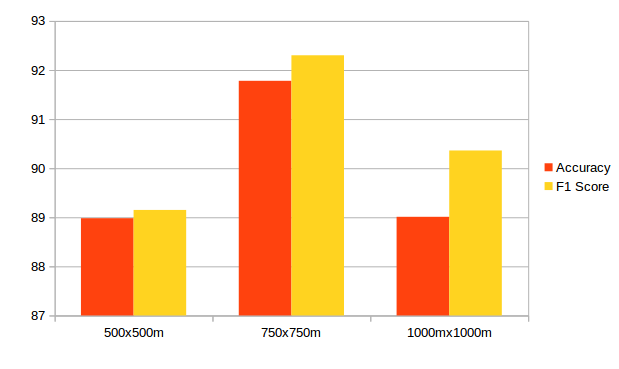
\includegraphics[width=0.6\textwidth]{dimensions-experiments}
    \caption{Results of  the experiments under different cell dimensions}
    \end{figure}

    The figure above shows that the LSTM network performed better when the grid uses 750mx750m cell dimension. Also, the network performs fairly in 1000mx1000m cell dimension and worst using 500mx500m cell dimension.

    \begin{figure}[ht]
    \centering
    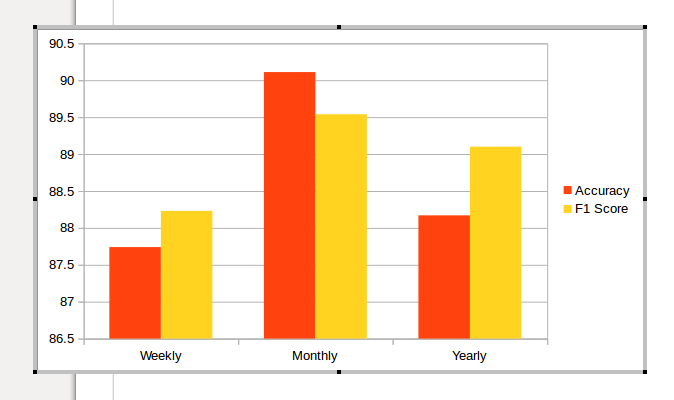
\includegraphics[width=0.6\textwidth]{timestep-experiment}
    \caption{Results of  the experiments under different timestep}
    \end{figure}

    In the next set of experiments, the LSTM network performs best using the monthly timestep. It performs second-best using the yearly timestep and worst using the weekly timestep.

    \begin{figure}[ht]
    \centering
    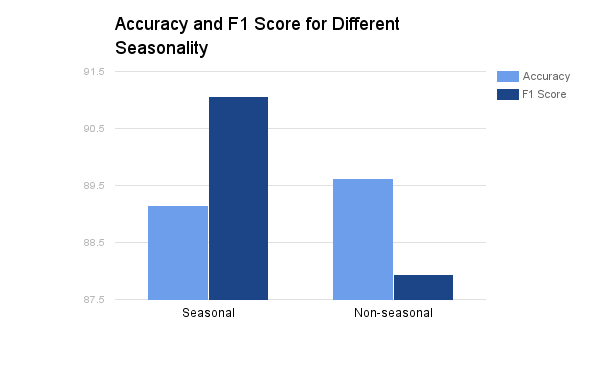
\includegraphics[width=0.6\textwidth]{seasonal-experiments}
    \caption{Results of  the experiments under seasonal and non-seasonal data}
    \end{figure}

    Between seasonal and non-seasonal data, the LSTM network works slightly better using the seasonal data.

    The results were analyzed by evaluating the performance of the model through error analysis. The learning curves of the model are shown below.

    \begin{figure}
    \label{fig:dimension-learning-curve}
    \centering     %%% not \center
    \subfigure[Figure A]{\label{fig:a}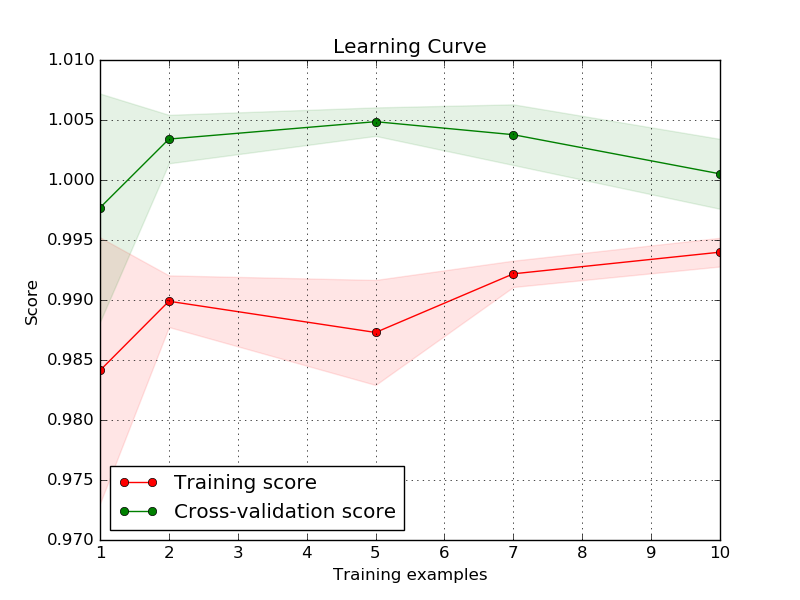
\includegraphics[width=.4\linewidth]{500-yearly}}
    \subfigure[Figure B]{\label{fig:b}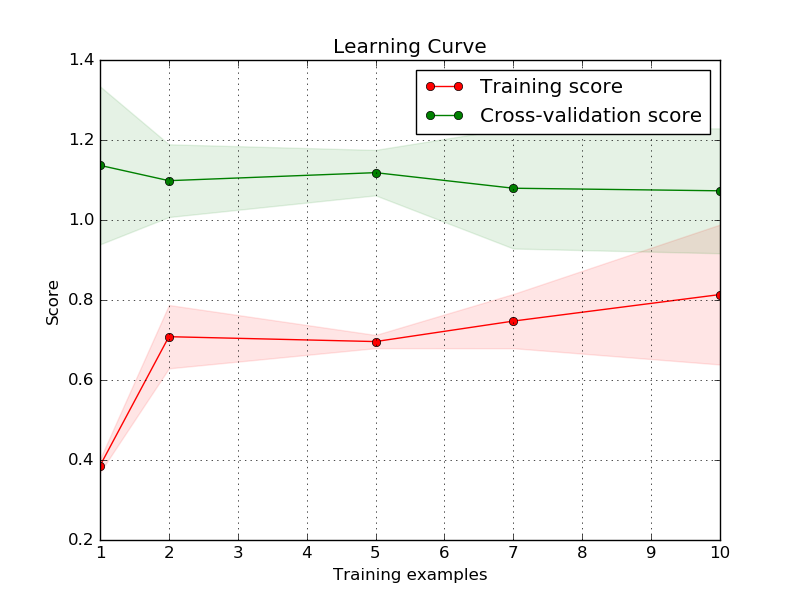
\includegraphics[width=.4\linewidth]{1000-yearly}}
    \caption{Learning curves of the model in different cell dimensions for the same timestep}
    \end{figure}

    The figure above shows the different learning curves of the model in different cell dimensions for the same timestep. The behavior of the training error and cross-validation error in both learning curves are almost similar, they tend to converge at the end but they have big gaps between them. Both instances of the model suffer from high variance. This may be because the yearly timestep yields only up to 16 samples with only 10 available for training. This low training sample size makes the model overfit. The graph shows that the variance or bias of the model is not affected by the cell dimension used.

    \begin{figure}
      \centering
      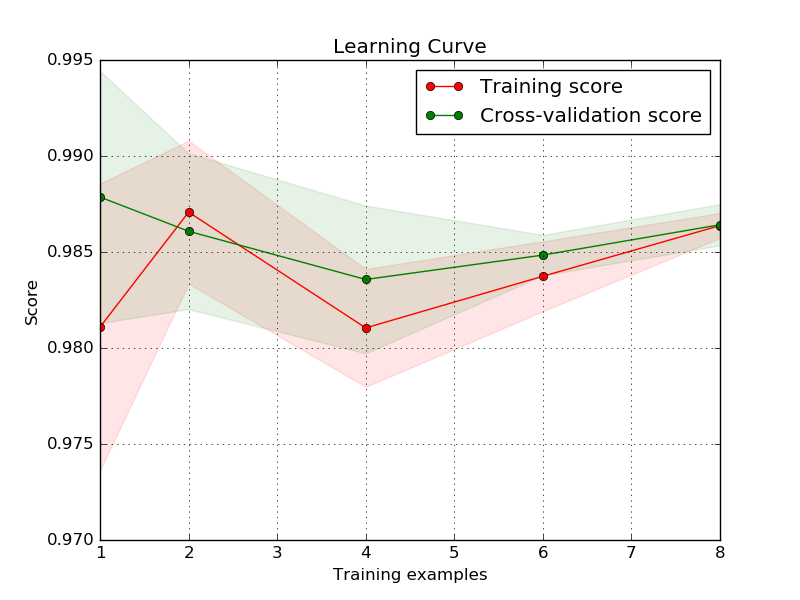
\includegraphics[width=0.5\textwidth]{1000_weekly_False}
      \caption{Learning curve of the model in 1000mx1000m cell dimension and weekly timestep}
      \label{fig:learning-curve2}
    \end{figure}

    Figure \ref{fig:learning-curve2} shows the graph of the training error and cross-validation error of the model in a 1000mx1000m cell dimension and weekly timestep. Compared to the same model but with yearly timestep, this model suffers from high bias. The training error and cross-validation overlap each other and are almost of the same value. Weekly timestep, on the contrary to yearly timestep, yields a lot of data with respect to the number of features used. The model under this condition will underfit and fail to generalize the data. To reduce underfitting, more features must be fed to the model so that it can have more input to help it generalize data better.

    \section {Conclusions and Recommendations}
    The model trained better using the cell dimension 750mx750m, monthly timestep and seasonal data. For a relatively new model in this field of application and using just one input, the LSTM model did reasonably well. Improvements could be done though according to the results of the error analysis. The model overfits when using the yearly timestep because there is no enough data. A yearly timestep could only be done if the data spans a longer period of years. Otherwise, other timesteps could be used. The model underifts though when using the weekly timestep. In this case, our model needs more features to help generalize data better. The model should be flexible enough for the different parameter values of timestep and seasonality. If the end-user of user wishes to predict crime hotspots weekly, or even daily, additional features must be introduced. The dataset contains other data that can be used as features for the model. For instance, a criminal record has a location type attribute that describes the nature of the location of the crime. It may be a street, apartment or other land mark. The yearly timestep can best be used when the data spans enough years for the model to avoid overfitting. There are other kinds of architecture of Recurrent Neural Networks, such as a Gated Recurrent Unit (GRU). It would also be worthwhile to investigate the performance of these implementations. There are also variations of Long Short-term Memory units. An example is the variation by Alex Graves, which is more suitable to sequence labelling and time series data.

    \end{multicols}
\end{document}